\part{Data analysis}
\label{part:data_analysis}

%------------------------------------

\section{About this part}
\label{section:DA_about_part}
Before rigorously testing different models available, it's important to take a look at the data that is supplied. The supplied data consists of 2 main groups of images, labelled training images and unlabeled test images.
As per the requirements of the Kaggle competition, the test images should only be used for evaluating the model on the Kaggle page by submitting a CSV of the prediction results.
Thus the test images can't be used for creating the model in any shape or form.
This means that only the labelled training images can be used to create and validate the model in development.
To avoid altering the model to perform well on the supplied test data and not in general, only the training data will be analysed.
All code used for this part is available under the developed code folder on GitHub, in the Jupyter Notebook \emph{data\_analysis.ipynb}.
This part describes how data can be analysed with the given code.
This code can be easily changed to analyse other variations of the data, e.g. using another descriptor.

%------------------------------------

\section{Data distribution}
\label{section:DA_data_distribution}
The provided labeled training data consists of 12 different classes.
There is a total of 4042 labelled training images supplied, the distribution of which is shown in figure \ref{fig:1-data_analysis-labeled_data_distribution}.
As visible in this figure, the distribution between classes is not balanced.
This has to be taken into account when fitting a model since some models will show unwanted behaviour when fitted with unbalanced data.
Luckily many solutions exist to minify the impact of this unbalance.


\begin{figure}[H]
    \centering
    \fbox{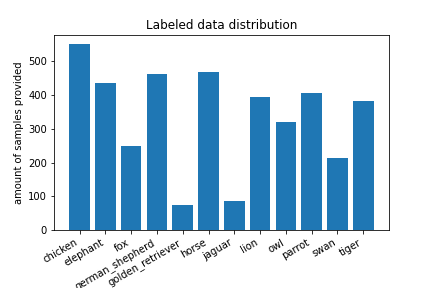
\includegraphics[width=0.8\linewidth]{images/1-data_analysis-labeled_data_distribution.png}}
    \captionsetup{width=0.7\linewidth}
    \captionsetup{justification=centering}
    \caption{The data distribution of the supplied training set.}
    \label{fig:1-data_analysis-labeled_data_distribution}
\end{figure}

%------------------------------------

\section{Deeper look at the training data}
\label{section:DA_deeper_look_data}

Whilst noting that the available data isn't balanced over all the classes is very important, there are also different aspects of the data that need analysing. 
An overview of the supplied training data is given in figure \ref{fig:1-data_analysis-labeled_data_overview.png}, available in the figures list at the end of this report.
This figure shows the first five images of each class.
From this, it becomes apparent that multiple factors of the data aren't \emph{optimal}.
This knowledge is important since it can aid in better prepossessing and in finding a better model in general.
The most noteworthy findings are listed here:
\begin{itemize}
    \item Images vary in shapes, some are taken in portrait, others in landscape.
    \item Images vary in size, some are high resolution whilst others are relatively low resolution.
    \item The framing of the subject(s) varies a lot. Sometimes the labelled animal is completely visible and centred in the frame. In some images there are multiple animals spread across the image, others show a close-up of the animal.
    \item Some images have a detailed background that makes up for a lot of the image, in others the background is blurry and its impact is presumably less.
    \item Some images have very vibrant colours in broad daylight, others are black and white in dimly lit environments.
\end{itemize}

This diversity in the provided training set is expected since it has been scraped from the web.
This also means that \emph{noise} can be expected, another important factor to keep in mind when choosing and optimizing models.
Many of the listed things can be minified by doing some clever prepossessing of the images.


%------------------------------------

\section{Feature extraction}
\label{section:DA_feature_extraction}

Since the focus of this competition is on developing great models and not necessarily on data prepossessing and feature extraction, some feature extraction has already been provided.
More info on the prepossessing and feature extraction provided is available in the provided notebook \emph{creating\_vbow.ipynb}.
In short, images are converted from there typical RGB representation to a numerical representation of interesting points, which can be used as input for our model.
How this is done will briefly be discussed here.

Instead of using the whole image as data, only a select few of \emph{interesting points} of the image are taken into consideration.
These interesting points of an image are found by using the \emph{Shi-Tomasi corner detector}.
The following important parameters for the \emph{features.extractShiTomasiCorners} function call are used for the supplied features:
\begin{itemize}
    \item number of features = 500
    \item minimum distance between features = 20
\end{itemize}

Shown in figure \ref{fig:1-data_analysis-POI} is an example output of interesting points found by the Shi-Tomasi corner detector.
It's clear that this is far from optimal, but finding interesting points isn't an easy task and thus the results are better then they might seem on first sight. 

\begin{figure}[H]
    \centering
    \fbox{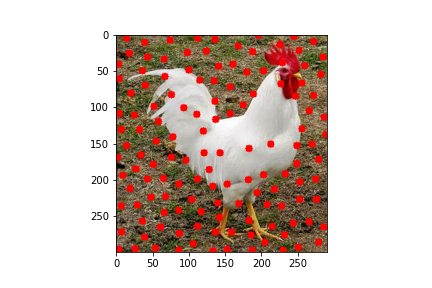
\includegraphics[width=0.8\linewidth]{images/1-data_analysis-POI.png}}
    \captionsetup{width=0.7\linewidth}
    \captionsetup{justification=centering}
    \caption{Example of points of interest found by Shi-Tomasi corner detector.}
    \label{fig:1-data_analysis-POI}
\end{figure}

Finding interesting points is only half of the work.
These interesting points now need to be represented by numerical values that have actual meaning.
Remember from section \ref{section:DA_deeper_look_data} that the provided images differ a lot and thus a descriptor has to be used that minifies the impact of different lighting, scaling...
The following descriptors are used and their outputs are provided: DAISY, ORB, FREAK, LUCID, VGG, BoostDesc, SIFT.
Whilst SURF is another great descriptor, it's not provided nor is the license available for this project.
SIFT is often referred to as the most famous and successful of these descriptors, but all of them should be explored.


%------------------------------------

\section{The numerical representation}
\label{section:DA_numerical_representation}

As discussed in section \ref{section:DA_feature_extraction}, the images are stored as numerical representations of different features using descriptors.
To save time, these numerical representations for all the descriptors are stored in a separate \emph{Pickle} file.
Since these representations form the input of a model, it's important to get a grip on how these look.
The provided \emph{createCodebook} function allows for easily loading in this data.
It also allows specifying how many features per image are wanted with the \emph{codebook\_size} parameter.
As discussed in section \ref{section:DA_feature_extraction}, at most 500 of these are available per image by default.
The function returns 2 lists, one containing the labels for the image represented at a certain index, the other containing the requested amount of features per image. 

An overview of the data from such features given by the SIFT descriptor is given in figure \ref{fig:1-data_analysis-labeled_data_overview.png}, available in the figures list at the end of this report.
From this, it is visible that the values seem to be normalized by the SIFT descriptor.
This would have to be checked for all descriptors used and perhaps some outliers would need to be removed.

In figure \ref{fig:1-data_analysis-correlation_matrix} the correlation matrix is shown for the first 30 features of the SIFT descriptor.
The correlation between these values doesn't seem too dramatic, which is mostly positive for our model building.

\begin{figure}[H]
    \centering
    \fbox{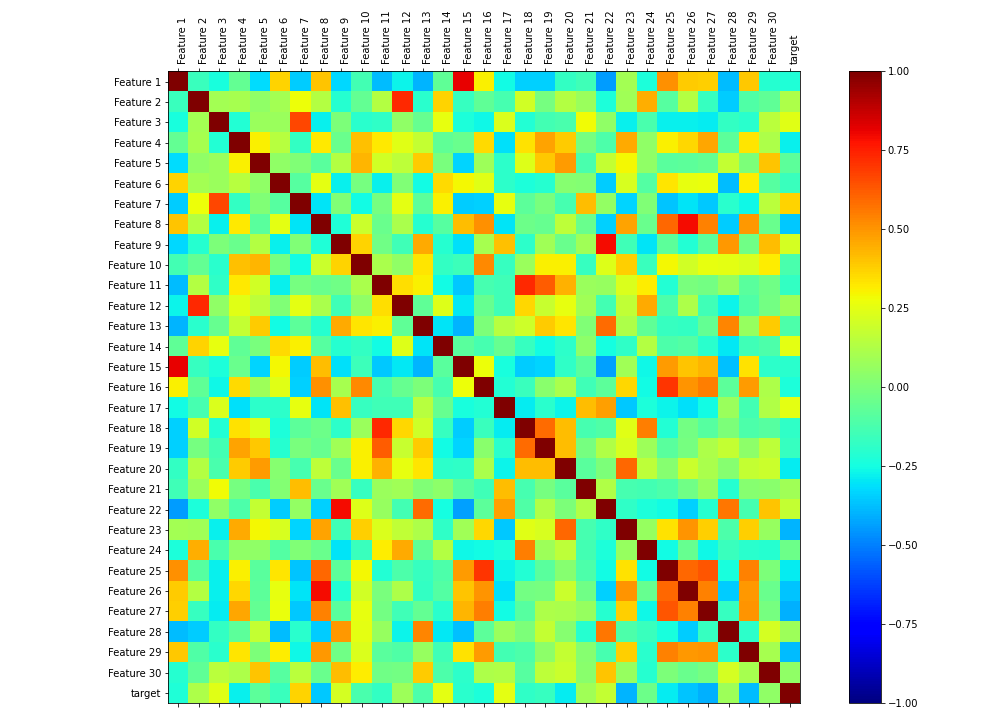
\includegraphics[width=0.8\linewidth]{images/1-data_analysis-correlation_matrix.png}}
    \captionsetup{width=0.7\linewidth}
    \captionsetup{justification=centering}
    \caption{Example of points of interest found by Shi-Tomasi corner detector.}
    \label{fig:1-data_analysis-correlation_matrix}
\end{figure}